\documentclass{article}
\usepackage{amsmath}
\usepackage{amssymb}
\usepackage{graphicx}
\usepackage{hyperref}
\usepackage[version=4]{mhchem}

\title{Problem 9}
\date{}

\begin{document}
\maketitle

\section*{Problem}
Diagonals \(A C\) and \(B D\) of quadrilateral \(A B C D\) meet at \(E\). If \(A E=2, B E\) \(=5, C E=10, D E=4\), and \(B C=15 / 2\), find \(A B\).\\
\centering
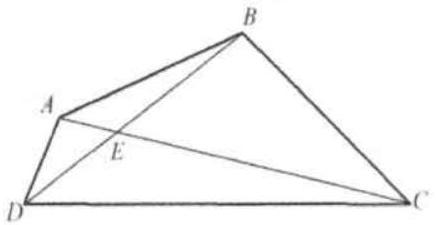
\includegraphics[width=\textwidth]{images/problem_image_1.jpg}

\section*{Solution}
\(\frac{1}{2} \sqrt{171}\).\\
As shown in the figure, since \(B E / A E=C E / D E=5 / 2, \triangle A E D \sim \triangle B E C\). Therefore, \(B E / A E=B C / A D\), or \(\frac{5}{2}=\frac{\frac{15}{2}}{A D}\).\\
Thus, \(A D=3\).\\
Similarly, \(\triangle A E B \sim \triangle D E C\).\\
Therefore, \(A E / D E=A B / D C\) or \(1 / 2=A B / D C\).\\
Thus, \(D C=2(A B)\).\\
Also, \(\angle \mathrm{L} B A C=\angle B D C\). Therefore, quadrilateral ABCD is cyclic.\\
Now, applying Ptolemy's Theorem to cyclic quadrilateral\\
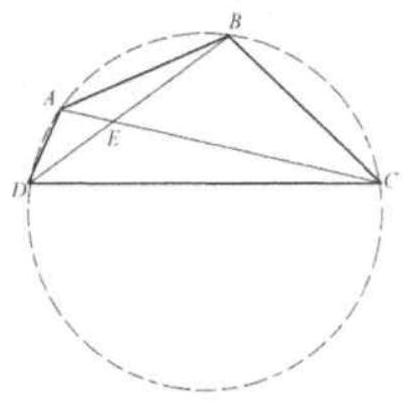
\includegraphics[width=\textwidth]{images/reasoning_image_1.jpg} \(A B C D\), \((A B)(D C)+(A D)(B C)=(A C)(B D)\).\\
Substituting, we find that \(A B=\frac{1}{2} \sqrt{171}\).

\end{document}
